\chapter{Evaluation the radiation of the sources}\label{radiation}
FAINA allows to evaluate electromagnetic radiation from sources with various type of particle distributions and different parameters such ass magnetic fiels, number density and other. In current version of the code following types of radiation are implemented: synchrotron radiation, inverse Compton scattering, gamma-ray emission due to pion decay in free-free proton interaction and also bremsstrahlung.

\section{Particle distributions}

Crucial parameter for evaluation of any type of radiation is a distribution function of emitting particles. In the FAINA code abstract class ParticleDistribution and derived classes are used for representation of distributions. Public methods of class ParticleDistribution are listed in Table \ref{ParticleDistribution}:

\begin{small}
		\topcaption{Public methods of ParticleDistribution class}
		\label{ParticleDistribution}
		
		\begin{xtabular}{|p{0.45\textwidth}|p{0.55\textwidth}|}
			\hline
			\textbf{ParticleDistribution} & abstract class for particle distributions\\
			\hline
			double distribution(const double\& energy, const double\& mu, const double\& phi) & returns probability density function in polar coordinates with given energy, cosinus of polar angle and azimutal angle, normalized to the particles number density \\
			\hline
			virtual double distributionNormalized(const double\& energy, const double\& mu, const double\& phi) & virtual method, returns probability density function in polar coordinates with given energy, cosinus of polar angle and azimutal angle, normalized to unity\\
			\hline
			virtual double getMeanEnergy() & virtual method, returns mean energy of particles in distribution\\
			\hline
			double getConcentration() & returns particles number density\\
			\hline
			void resetConcentration(const double\& concentration) & changes number density to the given value\\
			\hline
		\end{xtabular}
\end{small}

For creating a distribution object you need some inherited class. Inheritance tree of ParticleDistribution splits into two big branches - PhotonDistribution for distribution of photons, and MassiveParticleDistribution - for massive particles. Scheme of class hierarchy is shown in Figure  \ref{particleDistribution0}. 

\begin{figure}
	\centering
	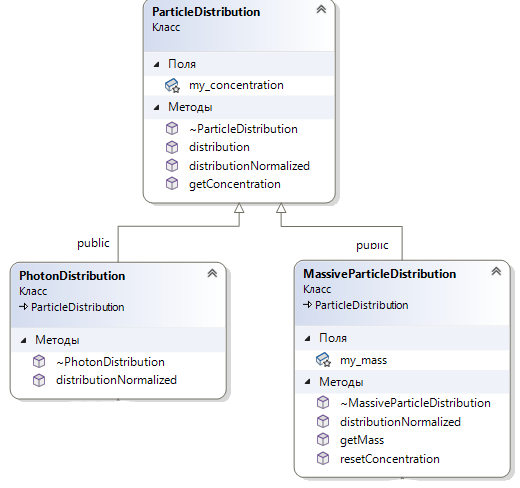
\includegraphics[width=8.5 cm]{./fig/particleDistribution0.png} 
	\caption{Two branches of inheritance tree of ParticleDIstribution}
	\label{particleDistribution0}
\end{figure}

It is important to note, that photons distributions are not used to represent results of evaluation of electromagnetic radiation. They are necessary only as input parameter for evaluation of inverse Compton scattering. Class PhotonDistribution is only an interface and has not its own specific methods. Class MassiveParticleDistribution is also abstract, but his methods are listed in Table \ref{MassiveParticleDistribution}	
\begin{small}
		\topcaption{Public methos of MassiveParticleDistribution class}
		\label{MassiveParticleDistribution}
		
			\begin{xtabular}{|p{0.45\textwidth}|p{0.55\textwidth}|}
				\hline
				\textbf{MassiveParticleDistribution} & abstract class for massive particles distribution\\
				\hline
				virtual double minEnergy() & virtual method, returns the lowest possible energy of particle in this distribution\\
				\hline
				virtual double maxEnergy() & 
				virtual method, returns the upper limit of energy of particle in this distribution. NOTE that if upper limit of energy is infinite, this method returns negative number\\
				\hline
				double getMass() & returns mass of single particle \\
				\hline
			\end{xtabular}
		\end{small}
\subsection{Photon distributions}

Abstract class PhotonDistribution has following derived class: abstract PhotonIsotropicDistribution, which represented isotopic distributions and some non-abstract classes: PhotonPlankDirectedDistribution, which represent photons with Plank distribution with respect to energy, but collimated in some solid angle, and CompoundPhotonDistribution, which is usefull for sum of several arbitrary photon distributions.

Class PhotonIsotropicDistribution again has its own inherited classes. It is a PhotonPowerLawDistribution for powerlaw distribution, PhotonPlankDistribution for Plank distributions, PhotonMultiPlankDistribution for sum of several Plank distributions and PhotonMonoenergeticDistribution for isotropic photons with same energy. Class hoerarchy of photon distributions is presented in Figure \ref{photonDistribution}.

\begin{figure}
	\centering
	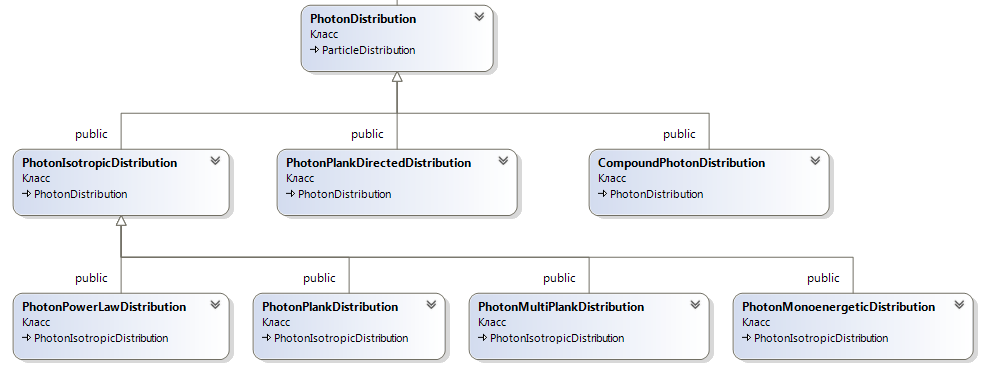
\includegraphics[width=10.5 cm]{./fig/photonDistribution2.png} 
	\caption{Class hierarchy of photon distributions}
	\label{photonDistribution}
\end{figure}

Methods of PhotonDistribution and it's inherited classes are listed in Table \ref{photonDistributionMethods}. NOTE, that metods distributionNormalized(const double\& energy) and distribution(const double\& energy) are not distribution with respect to energy, but just full distribution with dropped angular arguments. So to obtain distribution with respect to energy one should multiply result of this functions by $4\pi$.


\begin{small}
	\topcaption{Public methods of PhotonDistribution class and derived classes}
	\label{photonDistributionMethods}
	\begin{xtabular}{|p{0.45\textwidth}|p{0.55\textwidth}|}
				\hline
				\textbf{PhotonDistribution} & abstract interface for photon distributions\\
				\hline
				\textbf{PhotonIsotropicDistribution} & abstract class for isotropic distributions of photons\\
				\hline
				double distribution(const double\& energy) & returns probability density function in polar coordinates with dropped angular arguments (normalized to the number density divided by $4\pi$)\\
				\hline
				virtual double distributionNormalized(const double\& energy) & virtual method, returns probability density function in polar coordinates with dropped angular arguments (mormalized to the $1/4\pi$)\\
				\hline
				void writeDistribution(const char* fileName, int Ne, const double\& Emin, const double\& Emax) & writes distribution into given file as to columns - energy and distribution from Emin to Emax with Ne logarithmically distributed points\\
				\hline
				\textbf{PhotonPowerLawDistribution} & class representing powerlaw distribution of photons\\
				\hline
				PhotonPowerLawDistribution(const double\& index, const double\& E0, const double\& concentration) & constructor, creates distribution with given power-law index p such as $F(E)~1/E^p$, starting energy and number density \\
				\hline
				double getIndex() & returns power-law index\\
				\hline
				double getE0() & returns starting energy of distribution\\
				\hline
				\textbf{PhotonPlankDistribution} & class representing Plank distribution\\
				\hline
				PhotonPlankDistribution(const double\& temperature, const double\& amplitude) & constructor, creates distribution with given temperature and amplitude - relation of number density to the number density of photons in equilibrium black-body radiation\\
				\hline
				static PhotonPlankDistribution* getCMBRadiation() & static method, returns object representing Cosmic Microwave Background Radiation (temperature $2.725~\rm K$, amplitude $1$)\\
				\hline
				double getTemperature() & returns temperature of distribution\\
				\hline
				\textbf{PhotonMultiPlankDistribution} & class representing sum of several Plank distributions\\
				\hline
				PhotonMultiPlankDistribution(int N, const double* const temperatures, const double* const amplitudes) & constructor, creates distribution constisting of N plank distributions with given temperatures and amplitudes\\
				\hline
				static PhotonMultiPlankDistribution* getGalacticField() & static method, returns object representing mean Galactic photon field described in \cite{Mathis1983}. This distribution consists of five plank components with temperatures $2.725K, 20K, 3000K, 4000K, 7000K$ and amplitudes $1.0, 4\cdot10^{-4}, 4\cdot10^{-13}, 1.65\cdot10^{-13}, 1.0\cdot10^{-14}$ respectively\\
				\hline
				\textbf{PhotonMonoenergeticDistribution} & class representing population of isotropic photons with close energy\\
				\hline
				PhotonMonoenergeticDistribution(const double\& Energy, const double\& halfWidth, const double\& concentration) & constructor, creates object with given mean energy, half-width of uniform distribution around mean energy and number density\\
				\hline
				\textbf{CompoundPhotonDistribution} & class representing sum of several arbitrary distributions\\
				\hline
				CompoundPhotonDistribution(int N, PhotonDistribution** distributions) & constructor, creates distribution consisting of N arbitrary distributions\\
				\hline
				CompoundPhotonDistribution( PhotonDistribution* dist1, PhotonDistribution* dist2) & constructor, creates distribution which is sum of two given distributions\\
				\hline
				CompoundPhotonDistribution( PhotonDistribution* dist1, PhotonDistribution* dist2, PhotonDistribution* dist3) & constructor, creats distribution which is sum of three given distributions\\
				\hline
				\textbf{PhotonPlankDirectedDistribution} & class representing distribution which is Plank-like with respect to energy, but collimated into given direction\\
				\hline
				PhotonPlankDirectedDistribution(const double\& temperature, const double\& amplitude, const double\& theta0, const double\& phi0, const double\& deltaTheta) & constructor, creates distribution with given temperature, amplitude, angles determining mean direction of photons and half-width angle of cone in which photons propagate\\
				\hline
				double getTemperature() & return temperature of distribution\\
				\hline
	\end{xtabular}
\end{small}

User can define other photons distribution, creating class inherited from PhotonDistribution or PhotonIsotropicDistribution and overriding virtual method distributionNormalized.


\subsection{Distributions of massive particles}
Distributions of massive particles are represented by class MassiveParticleDistribution and inherited classes. Similarly to the photon distributions, isotropic distrinutions are important type, represented by class
MassiveParticleIsotropicDistribution. This class also has methods distributionNormalized(const double\& energy) and distribution(const double\& energy), which are not distribution with respect to energy, but just full distribution with dropped angular arguments. So to obtain distribution with respect to energy one should multiply result of this functions by $4\pi$.

Abstract class of isotropic distributions has seven inherited classes for specific distributions: MassiveParticlePowerLawDistribution - for power-law distributions, MassiveParticleBrokenPowerLawDistribution - for double power-law distibutions with knee, MassiveParticlePowerLawCutoffDistribution - for power-law distributions with exponential cutoff, MassiveParticleMaxwellDistribution - for non-relativistic maxwellian distribution (but it use full energy, including rest energy), MassiveParticleMaxwellJuttnerDistribution - for Maxwell
-Juttner distribution, MassiveParticleTabulatedIsotropicDistribution - for arbitrary distributions, described with array of values and MassiveParticleMonoenergeticDistribution - for beam of particles with close energies. Also there are six anisotropic distributions, implemented in the code. MassiveParticleTabulatedPolarDistribution - for tabulated distribution with dependence on energy and polar angle, MassiveParticleAnisotropicDistribution - for arbitrary tabulated anisotropic distributions, MassiveParticleMonoenergeticDirectedDistribution - for distributions represented narrow beam of particles with close energies, MassiveParticleMovingDistribution - for transformation the distributions from one frame to another, CompoundMassiveParticleDistribution - for sum of arbitraty distributions and CompoundWeightedMassiveParticleDistribution - for weighted sum of arbitrary distributions. In some cases operating with relative weghts of distributions is more useful than with absolute concentrations. Class hierarchy of distributions of massive particles is shown in Figure \ref{massiveDistribution}.


\begin{figure}[h]
	\centering
	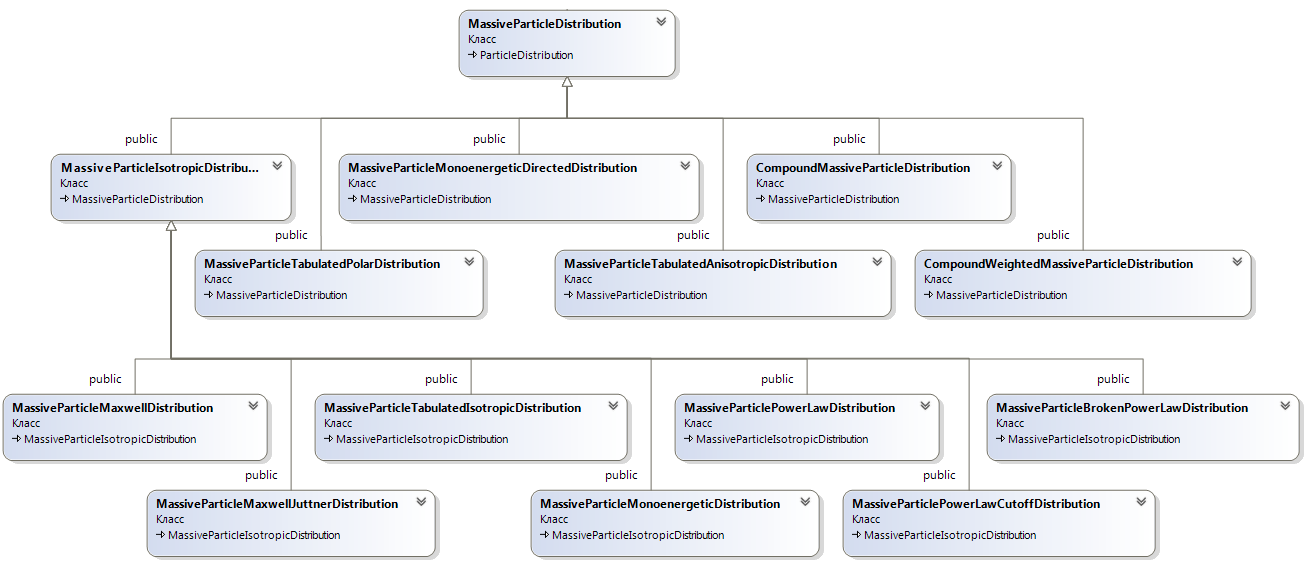
\includegraphics[width=14.5 cm]{./fig/massiveParticleDistribution2.png} 
	\caption{Class hierarchy of massive particles distributions}
	\label{massiveDistribution}
\end{figure}

public methods of classes for massive particle distributions are listed in Table \ref{MassiveParticleMethods}. User can define his own specific distributions, creating class inherited from MassiveParticleDistribution or MassiveParticleIsotropicDistribution.

\begin{small}
	\topcaption{Public methods of classes derived from MassiveParticleDistribution }
	\label{MassiveParticleMethods}
	\begin{xtabular}{|p{0.57\textwidth}|p{0.43\textwidth}|}				
		\hline
		\textbf{MassiveParticleIsotropicDistribution} & Abstract class for isotropic distributions of massive particles\\
		\hline
		double distribution(const double\& energy) & returns probability density function in polar coordinates with dropped angular arguments (normalized to the number density divided by $4\pi$)\\
		\hline
		virtual double distributionNormalized(const double\& energy) & virtual method, returns probability density function in polar coordinates with dropped angular arguments (mormalized to the $1/4\pi$)\\
		\hline
		void writeDistribution(const char* fileName, int Ne, const double\& Emin, const double\& Emax) &writes distribution into given file as to columns - energy and distribution from Emin to Emax with Ne logarithmically distributed points\\
		\hline
		double distributionNormalizedWithLosses( const double\& energy, const double\& lossRate, const double\& time) & returns a distribution which evaluted till time t via synchrotron losses with equation $f_t(E)=f\left(\frac{E}{1-E l t}\right)\cdot\frac{1}{\left(1- E l t\right)^2}$ and loss rate $l = 4e^4 B^2 /9m^4 c^7$\\
		\hline
		\textbf{MassiveParticlePowerLawDistribution} & class representibg power-law distribution\\
		\hline
		MassiveParticlePowerLawDistribution( const double\& mass, const double\& index, const double\& E0, const double\& concentration) & cobstructor, creates distribution with given particle mass, power-law index, starting energy and concentration\\
		\hline
		double getIndex() &returns power-law index\\
		\hline
		double getE0() & returns starting energy of distribution\\
		\hline
		\textbf{MassiveParticleBrokenPowerLawDistribution} & class representing double power-law distribution with knee\\
		\hline
		MassiveParticleBrokenPowerLawDistribution( const double\& mass, const double\& index1, const double\& index2, const double\& E0, const double\& Etran, const double\& concentration) & constructor, creates distribution with given particle mass, power-law indexes at low and high energies, starting energy, energy of transition from one index to another and concentration\\
		\hline
		double getIndex1() & returns power-law index at low energies\\
		\hline
		double getIndex2() & returns power-law index at high energies\\
		\hline
		double getE0() & returns starting energy of distribution\\
		\hline
		double getEtran() & returns energy of transition fron one index to another\\
		\hline
		\textbf{MassiveParticlePowerLawCutoffDistribution} & class representing power-law distribution with exponential cutoff\\
		\hline
		MassiveParticlePowerLawCutoffDistribution(const double\& mass, const double\& index, const double\& E0, const double\& beta, const double\& Ecut, const double\& concentration) & constructor, creates distribution with given particle mass, power-law index, starting energy, power of cutoff and cutoff energy and concentration $F(E)\propto (E/E_0)^{-index}\cdot\exp(-(E/E_{cut})^\beta)$\\
		\hline
		double getIndex() & returns power-law index \\
		\hline
		double getBeta() & returns cutoff power parameter \\
		\hline
		double getE0() & returns starting energy of distribution\\
		\hline
		double getEcutoff() & returns cutoff energy\\
		\hline
		\textbf{MassiveParticleMaxwellDistribution} & class representing non-relativistic maxwellian distribution\\
		\hline
		MassiveParticleMaxwellDistribution( const double\& mass, const double\& temperature, const double\& concentration) & creates distribution with given particles mass, temperature and concentration\\
		\hline
		double getTemperature() & returns temperature\\
		\hline
		\textbf{MassiveParticleMaxwellJuttnerDistribution} & class representing Maxwell-Juttner distribution\\
		\hline
		MassiveParticleMaxwellJuttnerDistribution( const double\& mass, const double\& temperature, const double\& concentration) & creates distribution with given particle mass, temperature and concentration\\
		\hline
		double getTemperature() & returns temperature\\
		\hline
		\textbf{MassiveParticleTabulatedIsotropicDistribution} & class for tabulated isotropic distribution\\
		\hline
		MassiveParticleTabulatedIsotropicDistribution( const double\& mass, const char* fileName, const int N, const double\& concentration, DistributionInputType inputType) & constructor, creates distribution with given mass and concentraion, reading table with N lines from given file. inpuType - enum variable determining in which coordinates distribution is defined in file\\
		\hline
		MassiveParticleTabulatedIsotropicDistribution( const double\& mass, const char* energyFileName, const char* distributionFileName, const int N, const double\& concentration, DistributionInputType inputType) & constructor, creates distribution with given mass and concentraion, reading Nx2 table with from two given files. inpuType - enum variable determining in which coordinates distribution is defined in files\\
		\hline
		MassiveParticleTabulatedIsotropicDistribution( const double\& mass, const double* energy, const double* distribution, const int N, const double\& concentration, DistributionInputType inputType) & constructor, creates distribution with given mass and concentraion, reading two data columns from given arrays. inpuType - enum variable determining in which coordinates distribution is defined in arrays\\
		\hline
		int getN() & returns number of grid points in distribution array\\
		\hline
		double rescaleDistribution(const double\& k) & rescales distribution through the energy axis using fourmula $E' = mc^2 + k\cdot(E-mc^2)$, $F(E')=F(E)/k$. It may be useful when e.g. distribution of electrons is obtained by numerical code with increased electron mass\\
		\hline
		void addPowerLaw( const double\& Epower, const double\& index) & replaces the tail of distribution with power-law distribution with given spectral index starting from Epower. Also renorms distribution\\
		\hline
		\textbf{MassiveParticleMonoenergeticDistribution} & class representing population of isotropic particles with close energy\\
		\hline
		MassiveParticleMonoenergeticDistribution(const double\& mass, const double\& Energy, const double\& halfWidth, const double\& concentration) & constructor, creates distribution with given particle mass, mean energy, half-width of uniform distribution around mean energy and number density\\
		\hline 
		\textbf{MassiveParticleTabulatedPolarDistribution} & class for tabulated distribution with dependence on energy and polar angle\\
		\hline
		MassiveParticleTabulatedPolarDistribution( const double\& mass, const char* energyFileName, const char* muFileName, const char* distributionFileName, const int Ne, const int Nmu, const double\& concentration, DistributionInputType inputType) & constuctor, creates distribution with given particle mass and concentration, reading it from files with energy grid points, angular grid points and distribution. inpuType - enum variable determining in which coordinates distribution is defined in files\\
		\hline
		MassiveParticleTabulatedPolarDistribution( const double\& mass, const double* energy, const double* mu, const double** distribution, const int Ne, const int Nmu, const double\& concentration, DistributionInputType inputType) & constuctor, creates distribution with given particle mass and concentration, using arrays with energy grid points, angular grid points and distribution. inpuType - enum variable determining in which coordinates distribution is defined in arrays\\
		\hline
		int getNe() & returns number of energy grid points in distribution array\\
		\hline
		int getNmu() & returns number of polar angle grid points in distribution array\\
		\hline
		void double rescaleDistribution(const double\& k) & 
		rescales distribution through the energy axis using fourmula $E' = mc^2 + k\cdot(E-mc^2)$, $F(E',\mu)=F(E,\mu)/k$. It may be useful when e.g. distribution of electrons is obtained by numerical code with increased electron mass\\
		\hline
		\textbf{MassiveParticleTabulatedAnisotropicDistribution} & class for arbitrary tabulated distribution\\
		\hline
		MassiveParticleTabulatedAnisotropicDistribution( const double\& mass, const char* energyFileName, const char* muFileName, const char* distributionFileName, const int Ne, const int Nmu, const int Nphi, const double\& concentration, DistributionInputType inputType) & constuctor, creates distribution with given particle mass and concentration, reading it from files with energy grid points, angular grid points and distribution. Grid with respect to azimuthal angle considered uniform and depends only on number of drid points Nphi. inpuType - enum variable determining in which coordinates distribution is defined in files\\
		\hline
		MassiveParticleTabulatedAnisotropicDistribution( const double\& mass, const double* energy, const double* mu, const double*** distribution, const int Ne, const int Nmu, const int Nphi, const double\& concentration, DistributionInputType inputType) & constuctor, creates distribution with given particle mass and concentration, using arrays with energy grid points, angular grid points and distribution. Grid with respect to azimuthal angle considered uniform and depends only on number of drid points Nphi. inpuType - enum variable determining in which coordinates distribution is defined in arrays\\
		\hline
		int getNe() & returns number of energy grid points in distribution array\\
		\hline
		int getNmu() & returns number of polar angle grid points in distribution array\\
		\hline
		int getNphi() & returns number of azimuthal angle grid points in distribution array\\
		\hline
		void rescaleDistribution(const double\& k) & rescales distribution through the energy axis using fourmula $E' = mc^2 + k\cdot(E-mc^2)$, $F(E',\mu, \phi)=F(E,\mu, \phi)/k$. It may be useful when e.g. distribution of electrons is obtained by numerical code with increased electron mass\\
		\hline
		\textbf{MassiveParticleMonoenergeticDirectedDistribution} & class representing narrow beam of particles with close energies\\
		\hline
		MassiveParticleMonoenergeticDirectedDistribution( const double\& mass, const double\& Energy, const double\& halfWidth, const double\& concentration, const double\& theta0, const double\& phi0, const double\& deltaTheta) & constructor, creates distribution with given particle mass, mean energy, half-width of uniform distribution around the mean energy, polar and azimuthal angles determining direction of mean velocity and half-width angle of velocity cone\\
		\hline
		\textbf{MassiveParticleMovingDistribution} & class transforming distribution from one frame to another\\
		\hline
		MassiveParticleMovingDistribution( MassiveParticleDistribution* distribution, const double\& velocity) & constructor, transforms the given distribution from the frame with givem velocity along z-axis to the lab frame\\
		\hline
		\textbf{CompoundMassiveParticleDistribution} & class representing distribution as sum of other distributions\\
		\hline
		CompoundMassiveParticleDistribution( int N, MassiveParticleDistribution** distributions) & constructor, creates distribution which is sum of given distributions\\
		\hline
		CompoundMassiveParticleDistribution( MassiveParticleDistribution* dist1, MassiveParticleDistribution* dist2) & constructor, creates distribution which is sum of two given distributions\\
		\hline
		CompoundMassiveParticleDistribution( MassiveParticleDistribution* dist1, MassiveParticleDistribution* dist2, MassiveParticleDistribution* dist3) & constructor, creates distribution which is sum of three given distributions\\
		\hline
		\textbf{CompoundWeightedMassiveParticleDistribution} & class representing distribution as weighted sum of other distributions\\
		\hline
		CompoundWeightedMassiveParticleDistribution( int N, const double* weights, MassiveParticleDistribution** distributions) & constructor, creates distribution which is sum of given distributions with given weights\\
		\hline
		CompoundWeightedMassiveParticleDistribution( MassiveParticleDistribution* dist1, const double\& w1, MassiveParticleDistribution* dist2, const double\& w2) & constructor, creates distribution which is sum of two given distributions with given weights\\
		\hline
		CompoundWeightedMassiveParticleDistribution( MassiveParticleDistribution* dist1, const double\& w1, MassiveParticleDistribution* dist2, const double\& w2, MassiveParticleDistribution* dist3, const double\& w3) & constructor, creates distribution which is sum of three given distributions with given weights\\
		\hline
		
	\end{xtabular}
\end{small}

\subsection{Reading distributions from file}
Classes for tabulated distribution, such as MassiveParticleTabulatedIsotropicDistribution, have constructors allowing to read distributions from files. It should be text files with tables of data, and format of data can be different. For determining data format there is enumerable type DistributionInputType with five possible values:

\begin{itemize}
	\item ENERGY\_FE - input file contains full energy in CGS units and distribution function $F(E)$
	\item ENERGY\_KIN\_FE - input file contains kinetic energy in CGS units and distribution function $F(E_{kin})$
	\item GAMMA\_FGAMMA - input file contains lorentz-factor and distribution function with respect to it $F(\gamma)$
	\item GAMMA\_KIN\_FGAMMA - input file contains reduced lorentz-factor ($\gamma - 1$) and distribution function with respect to it $F(\gamma-1)$
	\item MOMENTUM\_FP - input file contains momentum in CGS units and distribution function with respect to it $F(p)$
\end{itemize}

Regardless of input file format, distribution function would be transformed to the units energy vs distribution $F(E)$. Example of reading distribution from file is given below

\begin{lstlisting}[language=c++]
	double electronConcentration = 1.0;
	int N = 100;
	MassiveParticleIsotropicDistribution* distribution = new
	MassiveParticleTabulatedIsotropicDistribution(massElectron,
	"energy.dat", "distribution.dat", N, electronConcentration,
	DistributionInputType::ENERGY_FE);
\end{lstlisting}

Class MassiveParticleDistributionFactory is implemented for simplicity of reading distributions from files in complicated cases. It has several similar static methods allowing to read array of distribution from set of numerated files. It can be useful in cases when distribution function depends on some external parameter which varies inside the radiation source. Example of reading array of ten distributions of electrons from files, named "Fe0.dat"\ , "Fe1.dat"\ etc., consisting of two columns - loerntz-factor and distribution function, and adding power-law tail with index 3, starting from energy $10 m_e c^2$, calling one function is given below

\begin{lstlisting}[language=c++]
	double electronConcentration = 1.0;
	int Nenergy = 100;
	int Ndistribution = 100;
	double powerLawEnergy = 100*me_c2;
	double index = 3.0;
	MassiveParticleIsotropicDistribution** distributions = 
	MassiveParticleDistributionFactory::
	readTabulatedIsotropicDistributionsAddPowerLawTail(
	massElectron, "./input/Fe", ".dat", Ndistribution, 
	DistributionInputType::GAMMA_FGAMMA, electronConcentration, Nenergy,
	powerLawEnergy, index);
\end{lstlisting}

Also it is possible to create tabulated distributions not by reading them from files, but from arrays, which can be generated by user with any suitable method.

\section{Источники излучения}

В коде FAINA есть возможность расчета излучения, используя на прямую функции распределения излучающих частиц, с указанием необходимых дополнительных параметров, таких как объем источника, расстояние до него, магнитное поле и других. Но более универсальным и рекомендованным способ является расчет с помощью создания модели источника излучения. При таком подходе возможно учесть геометрическое строение источника, его неоднородности и другие особенности.

Реализованы два базовых класса источников - независящие от времени, представленные абстрактным классом RadiationSource, и изменяющиеся со временем, представленные абстрактным классом RadiationTimeDependentSource. Эти два класса не связаны между собой через наследование, но объект первого класса содержится внутри объектов второго как приватное поле класса. Схема классов источников излучения представлена на рисунке \ref{radiationSource}.

\begin{figure}[h]
	\centering
	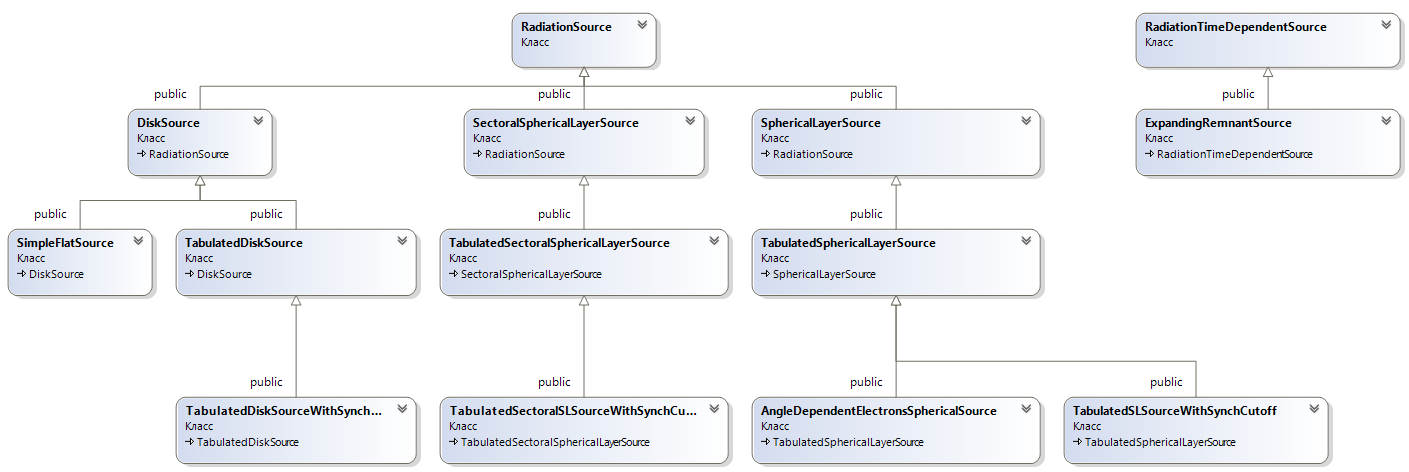
\includegraphics[width=14.5 cm]{./fig/radiationSource2.png} 
	\caption{Схема наследования классов источников излучения}
	\label{radiationSource}
\end{figure}

\subsection{Источники излучения, не зависящие от времени}\label{sourcesSection}
Источники излучения без временной зависимости реализованы с помощью абстрактного класса RadiationSource. Геометрически каждый источник задан в виде пространственной области в цилиндрических координатах, с осью z направленной вдоль луча зрения к наблюдателю, и характеризуется максимальным радиусом и минимальным и максимальным значением координаты z. Такая система координат выбрана для удобства учета процессов поглощения при прохождении излучения внутри самого источника вдоль луча зрения. Отличие реальной формы источника от цилиндрической реализовано с помощью долей заполнения веществом источника ячеек пространственной сетки. Модель источника, имеющего форму шарового слоя, в цилиндрическо пространственной сетке изображена на рисунке \ref{sphericalLayer}. Цветом обозначена доля объема ячейки, заполненная веществом источника.

\begin{figure}
	\centering
	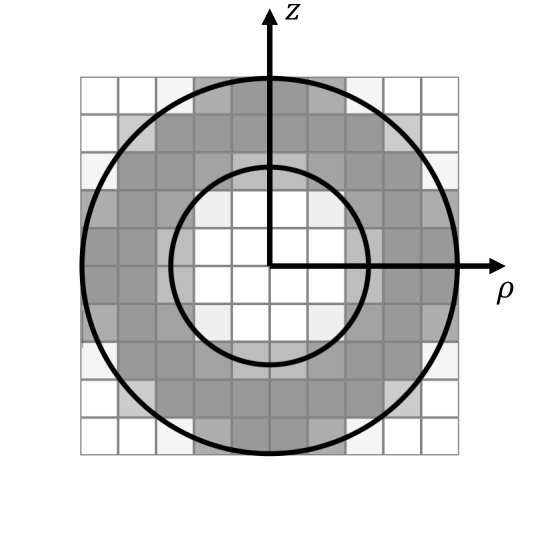
\includegraphics[width=10.5 cm]{./fig/sphericalSource.png} 
	\caption{Модель источника в форме шарового слоя, помещенного в цилиндрическую пространственную координатную сетку. Цвет характеризует долю объема ячейки, заполненную веществом источника.}
	\label{sphericalLayer}
\end{figure}

Так же источники излучения имеют следующие важные характеристки, которые могут меняться в различных пространственных ячейках источника: концентрация излучающих частиц, их функция распределения, магнитное поле и угол его наклона к лучу зрения. Большинство методов расчета излучения (все кроме обратного комптоновского рассеяния) реализованы только для изотропных распределений излучающих частиц, поэтому источники содержат только изотропные распределения. Так же у источника должно быть задано расстояние до наблюдателя.

Класс RadiationSource имеет три абстрактных класса-наследника: DiskSource - для источников в форме диска, перпендикулярного лучу зрения, и SphericalLayerSource - для источников в форме шарового слоя и SectoralSphericalLayerSource - источник, который нужен тогда, когда рассматривается только сектор шарового слоя, "долька апельсина". 

Источники в форме диска имеют три реализации: SimpleFlatSource - однородный диск, состоящий из одной пространственной ячейки с заданными параметрами, и TabulatedDiskSource - источник, в котором все характеристики таблично заданы на пространственной сетке и отнаследованный от него TabulatedDiskSourceWithSynchCutoff, который нужен для учета синхротронных потерь функции распределения. В можели данного источника считается, что распределение частиц генерирутся на границе источника (верхней грани, соответствующей ударной волне), а в дальнейшем конвекционно переносятся вглубь него, испытывая при этом синхротронные потери. Изменение функции распределения в зависимости от расстояния до границы в случае однородного поля определеяется формулой:

\begin{equation}
	f_l(E)=f\left(\frac{E}{1-4e^4 B^2 E~l/9m^4 c^7 v}\right)\cdot\frac{1}{\left(1-4e^4 B^2 E~l/9m^4 c^7 v\right)^2}
\end{equation}
где $f(E)$ исходная функция распределения, $E$ - энергия частицы, $B$ - магнитное поле, $l$ - расстояние до границы, $v$ - скорость конвекционного движения, $e$ - заряд частицы, $m$ - масса частицц, $c$ - скорость света.

Источники в форме шарового слоя имеют следующие реализации: TabulatedSphericalSource - источник, в котором все характеристики таблично заданы на пространственной сетке, и отнаследованные от него  TabulatedSLSourceWithSynchCutoff и AngleDependentElectronsSphericalSource. Первый из них нужен для учета синхротронных потерь, аналогично тому как это сделано в TabulatedDiskSourceWithSynchCutoff, а второй - для реализации важного случая, когда функция распределения излучающих частиц зависит от угла наклона магнитного поля по отношению к направлению распространения ударной волны \cite{SironiSpitkovsky2009pair, GuoSironi2014_1,Crumley2019, Romansky2018, еще}. В AngleDependentElectronsSphericalSource такие параметры, как концентрация, магнитное поле и его угол наклона к лучу зрения заданы таблично на пространственной сетке, а функция распределения излучающих частиц - в виде таблицы по углам наклона магнитного поля к направлению распространения ударной волны, которая в данном случае считается сферически симметричной. Функция распределения в каждой ячейке выбирается в зависимости от вычисленного угла наклона магнитного поля к ударной волне.

Источники в форме шарового слоя имеют следующие реализации: TabulatedSectoralSphericalLayerSource - источник, в котором все характеристики таблично заданы на пространственной сетке, и отнаследованный от него TabulatedSectoralSLSourceWithSynchCutoff, учитывающий потери энергии частиц аналогично тому, как это реализовано в классе TabulatedDiskSourceWithSynchCutoff.

Публичные методы классов источников излучения без зависимости от времени перечислены в Таблице \ref{sourceMethods1}.

\begin{small}
	\topcaption{Публичные методы классов источников излучения без зависимости от времени }
	\label{sourceMethods1}
	\begin{xtabular}{|p{0.5\textwidth}|p{0.5\textwidth}|}
		\hline
		\textbf{RadiationSource} & абстрактный класс для источников излучения общего вида\\
		\hline
		virtual double getMaxRho() & чисто виртуальный метод, возвращает границу источника по радиальной оси в цилиндрических координатах\\
		\hline
		virtual double getMinZ() & чисто виртуальный метод, возвращает минимальную границу источника по оси z\\
		\hline
		virtual double getMaxZ() & чисто виртуальный метод, возвращает максимальную границу источника по оси z\\
		\hline
		virtual double getMaxB() & чисто виртуальный метод, возвращает максимальное магнитное поле\\
		\hline
		virtual double getAverageSigma() & чисто виртуальный метод, возвращает среднюю магнетизацию $\sigma=\frac{B^2}{4\pi n m_p c^2}$\\
		\hline
		virtual double getAverageConcentration() &чисто виртуальный метод, возвращает среднюю конценрацию\\
		\hline
		virtual double getRho(int irho) & чисто виртуальный метод, возвращает радиальную координату данной ячейки\\
		\hline
		virtual double getZ(int iz)& чисто виртуальный метод, возвращает z координату данной ячейки\\
		\hline
		virtual double getPhi(int iphi)& чисто виртуальный метод, возвращает азимутальную координату данной ячейки\\
		\hline
		virtual int getRhoIndex(const double\& rho)& чисто виртуальный метод, возвращает радиальный индекс ячейки по координате\\
		\hline
		virtual bool isSource(int irho, int iphi)& чисто виртуальный метод, возвращает логическое значение - учитывать ли ячейки с данными радиальными и азимутальными координатами при расчете излучения всего источника\\
		\hline
		int getNrho() & возвращает количество пространственных ячеек по радиальной оси цилиндрических координат\\
		\hline
		int getNz() & возвращает количество пространственных ячеек по оси z цилиндрических координат\\
		\hline
		int getNphi() & возвращает количество пространственных ячеек по по азимутальному углу цилиндрических координат\\
		\hline
		double getDistance() & возвращает расстояние до источника\\
		\hline
		getArea(int irho) & возвращает поперечное сечение данной пространственной ячейки\\
		\hline
		getVolume(int irho, int iz, int iphi) & возвращает объем ячейки, занятый веществом источника. Этот метод согласован с методами getArea и getLength и возвращает их произведение\\
		\hline
		virtual getB(int irho, int iz, int iphi) & чисто виртуальный метод, возвращает значение магнитного поля в ячейке\\
		\hline
		virtual getConcentration(int irho, int iz, int iphi) & чисто виртуальный метод, возвращает значение концентрации в ячейке \\
		\hline
		virtual getSinTheta(int irho, int iz, int iphi) & чисто виртуальный метод, возвращает синус угла наклона магнитного поля к лучу зрения\\
		\hline
		virtual void getVelocity(int irho, int iz, int iphi, double\& velocity, double\& theta, double\& phi) &\\
		чисто виртуальный метод, возвращает скорость данной ячейки источника\\
		\hline
		virtual getTotalVolume() & чисто виртуальный метод, возвращает полный объем источника\\
		\hline
		virtual getLength(int irho, int iz, int iphi) & чисто виртуальный метод, возвращает среднюю толщину ячейки, заполненную веществом источника\\
		\hline
		virtual resetParameters(const double* parameters, const double* normalizationUnits) & чисто виртуальный метод, меняющий параметры источника. Список параметров, их количество, их влияние на источник определяются пользователем в конкретных реализациях класса. Принимет массив параметров и массив единиц в которых они измерены. Данный метод используется в процедурах оптимизации, либо при учете изменения источника со временем\\
		\hline
		virtual getParticleDistribution(int irho, int iz, int iphi) & чисто виртуальный метод, возвращает распределение излучающих частиц в ячейке\\
		\hline
		\textbf{DiskSource} & Абстрактный класс для источников в форме диска\\
		\hline
		\textbf{SimpleFlatSource} & Класс для источников в форме однородного диска\\
		\hline
		SimpleFlatSource( MassiveParticleDistribution* electronDistribution, const double\& B, const double\& sinTheta, const double\& rho, const double\& z, const double\& distance, const double\& velocity = 0) & конструктор, возвращает экземпляр с заданными распределением частиц, магнитным полем, синусом угла его наклона, радиусом диска, толщиной диска, расстоянием до источника и скоростью движения вещества\\
		\hline
		\textbf{TabulatedDiskSource} & Класс для источников в форме диска с таблично заданными значениями параметров\\
		\hline
		TabulatedDiskSource( int Nrho, int Nz, int Nphi, MassiveParticleDistribution* electronDistribution, double*** B, double*** sinTheta, double*** concentration, const double\& rho, const double\& z, const double\& distance, const double\& velocity = 0) & конструктор, возвращает экземпляр с заданными с помощью массивов распределением частиц, магнитным полем, синусом угла его наклона, а так же заданными радиусом диска, толщиной диска, расстоянием до источника и скоростью движения вещества\\
		\hline
		TabulatedDiskSource( int Nrho, int Nz, int Nphi, MassiveParticleDistribution* electronDistribution, const double\& B, const double\& sinTheta, const double\& concentration , const double\& rho, const double\& z, const double\& distance, const double\& velocity = 0) & конструктор, возвращает экземпляр с заданными однородными распределением частиц, магнитным полем, синусом угла его наклона, а так же заданными радиусом диска, толщиной диска, расстоянием до источника и скоростью движения вещества\\
		\hline
		\textbf{TabulatedDiskSourceWithSynchCutoff} & Класс для источников в форме диска с таблично заданными значениями параметров и учетом синхротронных потерь энергии частиц\\
		\hline
		TabulatedDiskSourceWithSynchCutoff(int Nrho, int Nz, int Nphi, MassiveParticleDistribution* electronDistribution, double*** B, double*** theta, double*** concentration, const double\& rho, const double\& z, const double\& distance, const double\& downstreamVelocity, const double\& velocity = 0) &
		конструктор, возвращает экземпляр с заданными с помощью массивов распределением частиц, магнитным полем, синусом угла его наклона, а так же заданными радиусом диска, толщиной диска, расстоянием до источника, скоростью конвекции частиц и скоростью движения вещества\\
		\hline
		TabulatedDiskSourceWithSynchCutoff(int Nrho, int Nz, int Nphi, MassiveParticleDistribution* electronDistribution, const double\& B, const double\& concentration, const double\& theta, const double\& rho, const double\& z, const double\& distance, const double\& downstreamVelocity, const double\& velocity = 0) & конструктор, возвращает экземпляр с заданными однородными распределением частиц, магнитным полем, синусом угла его наклона, а так же заданными радиусом диска, толщиной диска, расстоянием до источника, скоростью конвекции частиц и скоростью движения вещества\\
		\hline
		\textbf{SphericalLayerSource} & Абстрактный класс для источников в форме шарового слоя\\
		\hline
		double getInnerRho() & возвращает внутренний радиус шарового слоя\\
		\hline
		\textbf{TabulatedSphericalLayerSource} & Класс для источников в форме шарового слоя с таблично заданными значениями параметров\\
		\hline
		TabulatedSphericalLayerSource(int Nrho, int Nz, int Nphi, MassiveParticleDistribution* electronDistribution, double*** B, double*** sinTheta, double*** concentration, const double\& rho, const double\& rhoin, const double\& distance, const double\& velocity = 0) & конструктор, возвращает экземпляр с заданными с помощью массивов распределением частиц, магнитным полем, синусом угла его наклона к лучу зрения, а так же заданными внешним и внутренним радиусом шарового слоя, расстоянием до источника и скоростью движения вещества\\
		\hline
		TabulatedSphericalLayerSource(int Nrho, int Nz, int Nphi, MassiveParticleDistribution* electronDistribution, const double\& B, const double\& concentration, const double\& sinTheta, const double\& rho, const double\& rhoin, const double\& distance, const double\& velocity = 0) &  конструктор, возвращает экземпляр с заданными однородными распределением частиц, магнитным полем, синусом угла его наклона, а так же заданными внутренним и внешним радиусом шарового слоя, расстоянием до источника и скоростью движения вещества\\
		\hline
		\textbf{AngleDependentElectronsSphericalSource} & Класс для источников в форме шарового слоя с таблично заданными значениями концентрации и магнитного поля и функцией распределения излучающих частиц, зависящей от угла наклона магнитного поля к направлению распространения ударной волны\\
		\hline
		AngleDependentElectronsSphericalSource( int Nrho, int Nz, int Nphi, int Ntheta, MassiveParticleDistribution** electronDistributions, double*** B, double*** sinTheta, double*** phi, double*** concentration, const double\& rho, const double\& rhoin, const double\& distance, const double\& velocity = 0) & конструктор, возвращает экземпляр с заданными с помощью массивов магнитным полем, синусом угла его наклона к лучу зрения, а так же заданными внешним и внутренним радиусом шарового слоя, расстоянием до источника и скоростью движения вещества. Распределение частиц задается в виде массива табличных значений в зависимости от угла наклона магнитного поля к направлению распространения ударной волны\\
		\hline
		AngleDependentElectronsSphericalSource(int Nrho, int Nz, int Nphi, int Ntheta, MassiveParticleDistribution** electronDistributions, const double\& B, const double\& sinTheta, const double\& phi, const double\& concentration, const double\& rho, const double\& rhoin, const double\& distance, const double\& velocity = 0) & конструктор, возвращает экземпляр с заданными однородными  магнитным полем, синусом угла его наклона, а так же заданными внутренним и внешним радиусом шарового слоя, расстоянием до источника и скоростью движения вещества. Распределение частиц задается в виде массива табличных значений в зависимости от угла наклона магнитного поля к направлению распространения ударной волны\\
		\hline
		\textbf{TabulatedSLSourceWithSynchCutoff} & Класс для источников в форме шарового слоя с таблично заданными значениями параметров и учетом синхротронных потерь энергии частиц\\
		\hline
		TabulatedSLSourceWithSynchCutoff(int Nrho, int Nz, int Nphi, MassiveParticleDistribution* electronDistribution, double*** B, double*** theta, double*** concentration, const double\& rho, const double\& rhoin, const double\& distance, const double\& downstreamVelocity, const double\& velocity = 0) & конструктор, возвращает экземпляр с заданными с помощью массивов распределением частиц, магнитным полем, синусом угла его наклона к лучу зрения, а так же заданными внешним и внутренним радиусом шарового слоя, расстоянием до источника, скоростью конвекции частиц и скоростью движения вещества\\
		\hline
		TabulatedSLSourceWithSynchCutoff(int Nrho, int Nz, int Nphi, MassiveParticleDistribution* electronDistribution, const double\& B, const double\& concentration, const double\& theta, const double\& rho, const double\& rhoin, const double\& distance, const double\& downstreamVelocity, const double\& velocity = 0) & конструктор, возвращает экземпляр с заданными однородными распределением частиц, магнитным полем, синусом угла его наклона, а так же заданными внутренним и внешним радиусом шарового слоя, расстоянием до источника, скоростью конвекции частиц и скоростью движения вещества\\
		\hline
		\textbf{SectoralSphericalLayerSource} & абстрактный класс для источников в форме сектора шарового слоя (дольки апельсина)\\
		\hline
		double getRhoin() & возвращает внутренний радиус шарового слоя\\
		\hline
		\textbf{TabulatedSectoralSphericalLayerSource} & Класс для источников в форме сектора шарового слоя с таблично заданными значениями параметров\\
		\hline
		TabulatedSectoralSphericalLayerSource(int Nrho, int Nz, int Nphi, MassiveParticleDistribution* electronDistribution, double*** B, double*** theta, double*** concentration, const double\& rho, const double\& rhoin, const double\& minrho, const double\& phi, const double\& distance, const double\& velocity = 0) & конструктор, возвращает экземпляр с заданными с помощью массивов распределением частиц, магнитным полем, синусом угла его наклона к лучу зрения, а так же заданными внешним и внутренним радиусом шарового слоя, углом раствора сектора, расстоянием до источника и скоростью движения вещества\\
		TabulatedSectoralSphericalLayerSource(int Nrho, int Nz, int Nphi, MassiveParticleDistribution* electronDistribution, const double\& B, const double\& concentration, const double\& theta, const double\& rho, const double\& rhoin, const double\& minrho, const double\& phi, const double\& distance, const double\& velocity = 0) & конструктор, возвращает экземпляр с заданными однородными распределением частиц, магнитным полем, синусом угла его наклона, а так же заданными внутренним и внешним радиусом шарового слоя, углом раствора сектора, расстоянием до источника и скоростью движения вещества\\
		\hline
		\textbf{TabulatedSectoralSLSourceWithSynchCutoff} & Класс для источников в форме сектора шарового слоя с таблично заданными значениями параметров и учетом синхротронных потерь энергии частиц\\
		\hline
		TabulatedSectoralSLSourceWithSynchCutoff(int Nrho, int Nz, int Nphi, MassiveParticleDistribution* electronDistribution, double*** B, double*** theta, double*** concentration, const double\& rho, const double\& rhoin, const double\& minrho, const double\& phi, const double\& distance, const double\& downstreamVelocity, const double\& velocity = 0) & конструктор, возвращает экземпляр с заданными с помощью массивов распределением частиц, магнитным полем, синусом угла его наклона к лучу зрения, а так же заданными внешним и внутренним радиусом шарового слоя, углом раствора сектора, расстоянием до источника, скоростью конвекции частиц и скоростью движения вещества\\
		\hline
		TabulatedSectoralSLSourceWithSynchCutoff(int Nrho, int Nz, int Nphi, MassiveParticleDistribution* electronDistribution, const double\& B, const double\& concentration, const double\& theta, const double\& rho, const double\& rhoin, const double\& minrho, const double\& phi, const double\& distance, const double\& downstreamVelocity, const double\& velocity = 0) & конструктор, возвращает экземпляр с заданными однородными распределением частиц, магнитным полем, синусом угла его наклона, а так же заданными внутренним и внешним радиусом шарового слоя, углом раствора сектора, расстоянием до источника, скоростью конвекции частиц и скоростью движения вещества\\
		\hline
	\end{xtabular}
\end{small}

\subsection{Источники излучения, меняющиеся со временем}\label{timeDependentSource}
Источники излучения, учитывающие зависимость от времени, представлены абастрактным классом классом RadiationTimeDependentSource. Этот класс не является наследником класса RadiationSource, но содержит экземпляр такого класса внутри себя, чтобы использовать его для расчета излучения в конкретный момент времени. Для этого пользователь должен самостоятельно создать имплементацию виртуальной функции getRadiationSource, в которой будут вычислены параметры источника в зависимости от времени.  В текущей версии кода реализован только один наследник RadiationTimeDependentSource - ExpandingRemnantSource, представляющий собой модель расширяющегося остатка сверхновой. В данной модели предполагается, что размер источника увеличивается во времени с постоянной скоростью, магнитное поле падает обратно пропорционально размеру источника, концентрация обратно пропорционально квадрату размера а толщина шарового слоя остается постоянной. Пользователь может создавать свои классы источников с другими зависимостями параметров от времени. Публичные методы классов RadiationTimeDependentSource и ExpandingRemnantSource перечислены  в Таблице \ref{sourceTimeDependentMethods1}.

\begin{small}
	\topcaption{Публичные методы классов источников излучения учитывающих зависимость от времени }
	\label{sourceTimeDependentMethods1}
	\begin{xtabular}{|p{0.5\textwidth}|p{0.5\textwidth}|}
		\hline
		\textbf{RadiationTimeDependentSource} & Абстрактный класс для учета изменений источников излучения со временем\\
		\hline
		virtual resetParameters(const double* parameters, const double* normalizationUnits) & чисто виртуальный метод, меняющий параметры источника. Список параметров, их количество, их влияние на источник определяются пользователем в конкретных реализациях класса. Принимает массив параметров и массив единиц в которых они измерены. Данный метод применяется в процедурах оптимизации\\
		\hline
		virtual getRadiationSource(double\& time, const double* normalizationUnits) & возвращает источник излучения с параметрами соответствующими заданному моменту времени. Так же принимает на вход массив единиц, в которых измеряются параметры этого источника.\\
		\hline
		\textbf{ExpandingRemnantSource} & класс, представляющий модель расширяющегося с постоянной скоростью остатка сверхновой, имеющего форму шарового слоя постоянной толщины с однородными концентрацией и магнитным полем \\
		\hline
		ExpandingRemnantSource(const double\& R0, const double\& B0, const double\& concentration0, const double\& v, const double\& widthFraction, RadiationSource* source, const double\& t0) & конструктор, создает экземпляр класса расширяющейся сферической оболочки с заданными в момент t0 радиусом, магнитным полем, концентрацией, скоростью расширения, отношением толщины оболочки к радиусу и моделью источника. Для коректного учета изменения источника во времени важно, чтобы конретная реализация метода source->resetParameters соответствовала той,что используется в методе getRadiationSource. В данном случае подходят все перечисленные выше реализации источников не зависящих от времени\\
		\hline
	\end{xtabular}
\end{small}

\section{Вычисление излучения}

Для расчета излучения источников используется абстрактный класс RadiationEvaluator и его наследники, предназначенные для конкретных видов излучения. Так же есть класс RadiationSumEvaluator, предназначенный для суммирования нескольких различных видов излучения. Список публичных методов этих двух классов приведен в Таблице \ref{radiationEvaluator}. Общая схема расчета излучения такова: создать источник излучения, используя один из классов описанных в предыдущем разделе или написанный самостоятельно, затем создать вычислитель излучения нужного типа, и вызвать у него метод evaluateFluxFromSource(const double\& photonFinalEnergy, RadiationSource* source), вычисляющий энергетическую плотность потока излучения источника на данной энергии принимаемого фотона в единицах  $\text{см}^{-2} \text{с}^{-1}$. Далее в данном разделе описаны реализации класса RadiationEvaluator для конкретных видов излучения. Схема наследования классов вычислителей излучения представлена на рисунке \ref{radiationEvaluators}. Физическая сторона вопроса, формулы по которым расчитывается излучение подробно описаны в Главе \ref{Formulae}.

\begin{small}
	\topcaption{Публичные методы классa RadiationEvaluator }
	\label{radiationEvaluator}
	\begin{xtabular}{|p{0.5\textwidth}|p{0.5\textwidth}|} 
		\hline
		\textbf{RadiationEvaluator} & абстрактный класс для вычисления излучения \\
		\hline
		virtual evaluateFluxFromSource(const double\& photonFinalEnergy, RadiationSource* source) & чисто виртуальный метод, возвращает энергетическую плотность потока излучаемого данным источником в единицах $\text{см}^{-2} \text{с}^{-1}$ \\
		\hline
		virtual double evaluateFluxFromSourceAtPoint(const double\& photonFinalEnergy, RadiationSource* source, int rhoi, int phi) & чисто виртуальный метод, возвращает энергетическую плотность потока, излучаемого данной областью источника на картинной плоскости\\
		double evaluateTotalFluxInEnergyRange(const double\& Ephmin, const double\& Ephmax, int Nph, RadiationSource* source) & возвращает интегральны поток излучаемый источником в заданном диапазоне энергий (проинтегрированный по Nph точкам) в единицах  $\text{эрг} \text{см}^{-2} \text{с}^{-1}$\\
		\hline
		virtual resetParameters( const double* parameters, const double* normalizationUnits) & чисто виртуальный метод, позволяет изменить внутренние параметры вычислителя излучения. Список параметров, их количество, их влияние на источник определяются  в конкретных реализациях класса, данный метод используется при оптимизации\\
		\hline
		writeFluxFromSourceToFile(const char* fileName, RadiationSource* source, const double\& Ephmin, const double\& Ephmax, const int Nph) & записывает в файл с данным именем излучение источника в единицах $\text{см}^{-2} \text{с}^{-1}$ в диапазоне от минимальной до максимальной энергии, с заданным количеством точек, распределенных логарифмически\\
		\hline
		void writeImageFromSourceToFile(const char* fileName, RadiationSource* source, const double\& Ephmin, const double\& Ephmax, const int Nph) & записывает в файл с данным именем изображение - двумерный массив с интегральным потоком излучаемым разными областями источника в единицах $\text{эрг} \text{см}^{-2} \text{с}^{-1}$ в диапазоне от минимальной до максимальной энергии, проинтегрированым по заданныму количеству точек, распределенных логарифмически\\
		\hline
		void writeImageFromSourceAtEToFile(const double\& photonFinalEnergy, const char* fileName, RadiationSource* source) & записывает в файл с данным именем изображение - двумерный массив с энергетической плотностью потока излучаемого разными областями источника на данных энергиях в единицах $\text{см}^{-2} \text{с}^{-1}$\\
		\hline
		\textbf{RadiationSumEvaluator} & класс предназначенный для суммирования нескольких видов излучения\\
		\hline
		RadiationSumEvaluator(int Ne, const double\& Emin, const double\& Emax, RadiationEvaluator* evaluator1, RadiationEvaluator* evaluator2) & конструктор, создающий экземпляр с указанным диапазоном рассматриваемых энергий излучающих частиц, вычисляющий и складывающий результаты двух указанных вычислителей \\
		\hline
		RadiationSumEvaluator(int Ne, const double\& Emin, const double\& Emax, int Nev, RadiationEvaluator** evaluators) & конструктор, создающий экземпляр с указанным диапазоном рассматриваемых энергий излучающих частиц, вычисляющий и складывающий результаты вычислителей излучения в указанном массиве\\
		\hline
	\end{xtabular}
\end{small}

\begin{figure}[h]
	\centering
	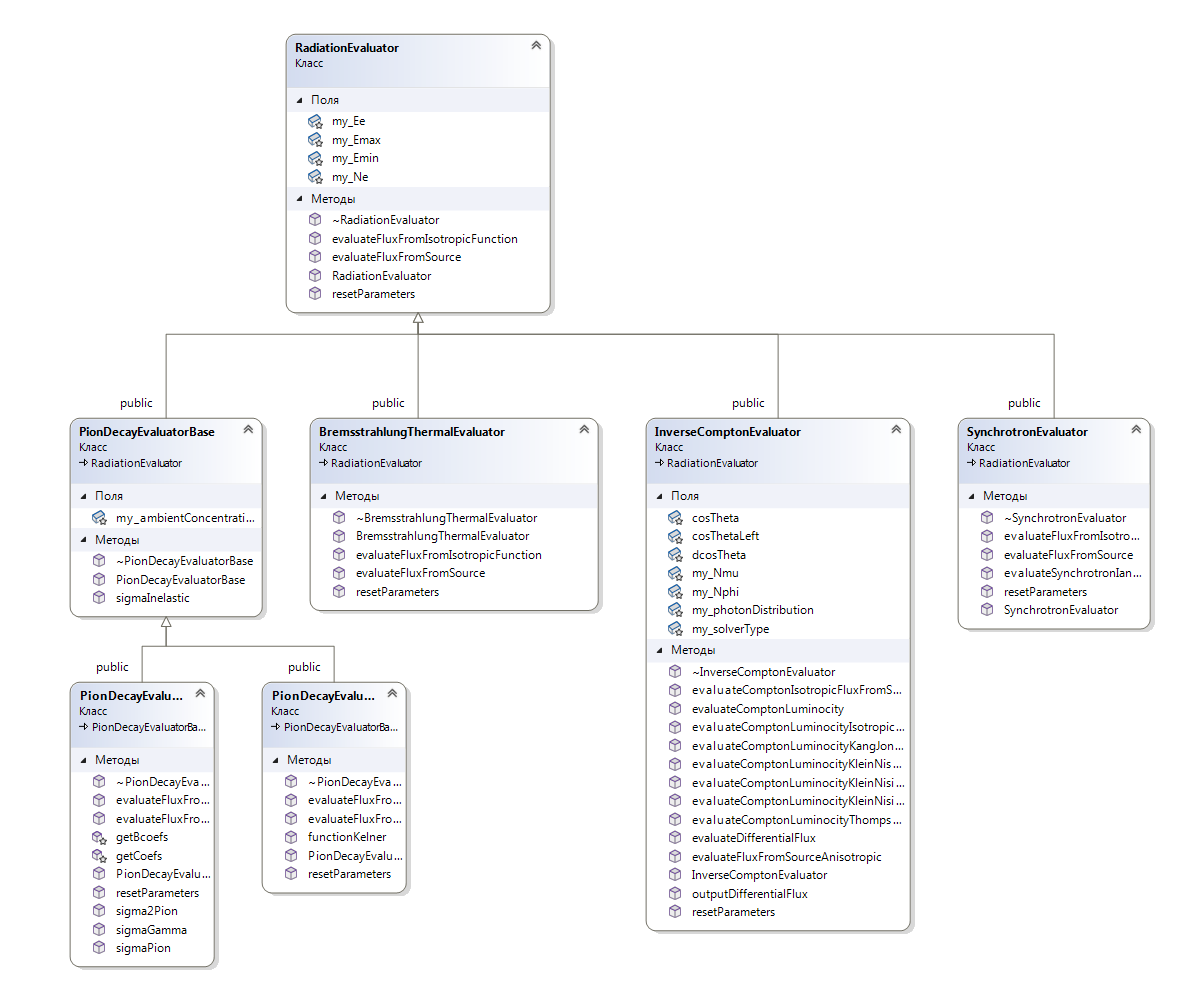
\includegraphics[width=10.5 cm]{./fig/radiationEvaluator.png} 
	\caption{Схема наследования классов вычислителей излучения.}
	\label{radiationEvaluators}
\end{figure}

\subsection{Синхротронное излучение}
Для расчета синхротронного излучения используется класс SynchrotronEvaluator. В нем используется приближение непрерывного спектра, то есть рассматриваемые частоты фотонов предполагаются намного большими, чем частота вращения излучающих частиц в магнитном поле. Реализован случай только изотропной функции распределения излучающих частиц. Так же возможен учет синхротронного самопоглощения. Используемая геометрия источников, показанная на рисунке \ref{sphericalLayer}, позволяет легко интегрировать излучение по лучу зрения, и учитывать при этом поглощение внутри источника. При создании объекта класса необходимо указать рассматриваемый диапазон энергий частиц и количество точек в нем, параметр отвечающий за учет самопоглощения (значение по умолчанию true), а так же значения магнитного поля, синуса угла наклона к лучу зрения и толщины излучаемой области, которые будут использоваться в случае расчета излучения без указания источника, а только с использованием распределения частиц. Публичные методы класса SynchrotronEvaluator перечислены в Таблице \ref{SynchrotronEvaluator}. Пример вычисления синхотронного излучения приведен в разделе \ref{quickStart}.
\begin{table}
	\begin{center}
	\begin{small}
	\caption{Публичные методы классa SynchrotronEvaluator }
	\label{SynchrotronEvaluator}
	\begin{tabularx}{\textwidth}{|X|X|} 
		\hline
		\textbf{SynchrotronEvaluator} & класс предназначенный для вычисления синхротронного излучения\\
		\hline
		SynchrotronEvaluator( int Ne, double Emin, double Emax, bool selfAbsorption = true, bool doppler = false) & конструктор, создает экземпляр с указанным диапазоном рассматриваемых энергий излучающих частиц,и параметрами учета самопоглощения и допплеровского эффекта\\
		\hline
		evaluateSynchrotronIandA(const double\& photonFinalFrequency, const double\& photonFinalTheta, const double\& photonFinalPhi, const double\& B, const double\& sinhi, const double\& concentration, MassiveParticleIsotropicDistribution* electronDistribution, double\& I, double\& A) & вычисляет значения плотности излучательной способности и коэффициента поглощения для фотона с данной энергией и направлением, в области с данными концентрацией и распределением излучающих частиц в данном магнитном поле\\
		\hline
	\end{tabularx}
\end{small}
\end{center}
\end{table}
\subsection{Обратное комптоновское рассеяние}
Для расчета излучения, получающегося в результате процесса обратного комптоновского рассеяния, использеуются классы InverseComptonEvaluator и его наследник InverseComptonEvaluatorWithSource. Отличие между ними в том, что в первом функция распределения рассеиваемых фотонов одинакова во всем излучающем объеме, а во втором изменяется обратно пропорционально квадрату расстояния до источника фотонов. Внутри класса  InverseComptonEvaluator реализованы четыре различных метода расчета излучения, для обозначения которых используется перечислимый тип ComptonSolverType, имеющий следующие значения:

\begin{itemize}
	\item ISOTROPIC\_THOMSON - модель рассеяния в томсоновсков режиме. Реализовано только для степенного распределения электронов и теплового фотонов \cite{Ginzburg1975} глава 17, с. 466
	\item ANISOTROPIC\_KLEIN\_NISHINA - модель расчитывающее излучение напрямую из сечения Клейна-Нишины, возможен учет анизотропных функций распределения \cite{KleinNishina, Dubus}
	\item ISOTROPIC\_KLEIN\_NISHINA - модель расчитывающее излучение напрямую из сечения Клейна-Нишины, но для изотропных функций распределения, что позволяет уменьшить количество интегрирований
	\item ISOTROPIC\_JONES - модель, использующая аналитически проинтегрированное по углам сечение Клейна-Нишины \cite{JonesCompton, BykovUvarov2000}
\end{itemize}

При создании объекта класса InverseComptonEvaluator необходимо указать рассматриваемый диапазон энергий частиц и количество точек в нем, количество ячеек в сетке по полярному и азимутальному углу, изотропную функцию распределения фотонов, которая будет использоваться по умолчанию и метод расчета излучения. Публичные методы классов InverseComptonEvaluator и InverseComptonEvaluatorWithSource перечислены в Таблице \ref{InverseComptonEvaluator}.
\begin{small}
	\topcaption{Публичные методы классa InverseComptonEvaluator }
	\label{InverseComptonEvaluator}
	\begin{xtabular}{|p{0.5\textwidth}|p{0.5\textwidth}|} 
		\hline
		\textbf{InverseComptonEvaluator} & класс предназначенный для вычисления излучения рождащегося в результате обратного комптоновского рассеяния\\
		\hline
		InverseComptonEvaluator( int Ne, int Nmu, int Nphi, double Emin, double Emax, PhotonDistribution* photonDistribution, ComptonSolverType solverType) & конструктор, создает экземпляр с заданным рассматриваемым диапазоном энергии, количеством ячеек в сетке по полярному и азимутальному углу, функцией распределения фотонов, которая будет использоваться по умолчанию и методом расчета излучения\\
		\hline
		evaluateComptonFluxKleinNishinaAnisotropic const double\& photonFinalEnergy, const double\& photonFinalTheta, const double\& photonFinalPhi, PhotonDistribution* photonDistribution, MassiveParticleDistribution* electronDistribution, const double\& volume, const double\& distance) & возвращает энергетическую плотность потока энергии в заданном направлении, излучением созданным заданными функциями распределения фотонов и рассеивющих частиц (которые могут быть анизотропными) в заданном объеме на данном расстоянии\\
		\hline
		evaluateFluxFromSourceAnisotropic( const double\& photonFinalEnergy, const double\& photonFinalTheta, const double\& photonFinalPhi, PhotonDistribution* photonDistribution, RadiationSource* source) & возвращает энергетическую плотность потока энергии в заданном направлении, излучением созданным заданными распределения фотонов и источником, содержащим распределения рассеивающих частиц\\
		\hline
		\textbf{InverseComptonEvaluatorWithSource} & класс предназначенный для вычисления излучения рождащегося в результате обратного комптоновского рассеяния с учетом зависимости функции распределения фотонов от расстояния до их источника\\
		\hline
		InverseComptonEvaluatorWithSource(int Ne, int Nmu, int Nphi, double Emin, double Emax, double Ephmin, double Ephmax, PhotonDistribution* photonDistribution, ComptonSolverType solverType, const double\& sourceR, const double\& sourceZ, const double\& sourcePhi) & конструктор, создает экземпляр с заданным рассматриваемым диапазоном энергии, количеством ячеек в сетке по полярному и азимутальному углу, функцией распределения фотонов, методом расчета излучения и координатами источника фотонов\\
		\hline
	\end{xtabular}
\end{small}

Пример вычисления излучения от обратного комптоновского рассеяние содержится в процедуре evaluateComtonWithPowerLawDistribution() в файле examples.cpp. В ней расчитывается рентгеновское излучение, исходящее от объекта CSS161010 при рассеивании степенного распределения электронов, определенного в работе \cite{Coppejans2020}, на среднегалактическом распределении фотонов.  Сначала определим переменные, задающие основные параметры источника - концентрацию частиц, его размер и магнитное поле. Для вычисления обратного комптоновского рассеяния магнитное поле не используется, но в источнике нужно его задать, поэтому положим его равным нулю. Так же зададим параметры сетки по энергиям и углам, которая будет использоваться вычислителем

\begin{lstlisting}[language=c++]
	double electronConcentration = 150;
	double sinTheta = 1.0;
	double rmax = 1.3E17;
	double B = 0.0;
	double distance = 150*1E6*parsec;
	
	double Emin = me_c2;
	double Emax = 1000 * me_c2;
	int Ne = 200;
	int Nmu = 20;
	int Nphi = 4;
\end{lstlisting}

Далее создадим распределение фотонов, воспользовавшись статическим методом класса MultiPlankDistribution getGalacticField, который возвращает среднегалактическое фотонное распределение, и распределение электронов - возьмем степенное рспределение с показателем 3.5.
\begin{lstlisting}[language=c++]
	PhotonIsotropicDistribution* photonDistribution = 
	    PhotonMultiPlankDistribution::getGalacticField();
	MassiveParticlePowerLawDistribution* electrons = new 
	    MassiveParticlePowerLawDistribution(massElectron, 3.5,
	    Emin, electronConcentration);
\end{lstlisting}

С помощью введенных ранее переменных создадим источник излучения и вычислитель излучения. В качестве метода расчета выберем самый универсальный - ANISOTROPIC\_KLEIN\_NISHINA

\begin{lstlisting}[language=c++]
	RadiationSource* source = new SimpleFlatSource(
	  electrons, B, sinTheta, rmax, rmax, distance);
	
	InverseComptonEvaluator* comptonEvaluator = new 
	    InverseComptonEvaluator(Ne, Nmu, Nphi, Emin, Emax, 
	    photonDistribution, ComptonSolverType::ANISOTROPIC_KLEIN_NISHINA);
\end{lstlisting}

Предположим, что мы не хотим пользоваться встроенным методом вывода излучения в файл, так как хотим получить конечный результат в других единицах, например энергию фотона измерять в электронвольтах, а поток вывести в формате $E F(E)$ - $\text{эрг}\text{см}^{-2}\text{с}^{-1}$. Создадим тогда сетку значений энергии фотонов
\begin{lstlisting}[language=c++]
	int Nnu = 200;
	double* E = new double[Nnu];
	double* F = new double[Nnu];
	double Ephmin = 0.01 * kBoltzman * 2.725;
	double Ephmax = 2 * Emax;
	double factor = pow(Ephmax / Ephmin, 1.0 / (Nnu - 1));
	E[0] = Ephmin;
	F[0] = 0;
	for (int i = 1; i < Nnu; ++i) {
		E[i] = E[i - 1] * factor;
		F[i] = 0;
	}
\end{lstlisting}
после этого вычислим в цикле желаемые потоки излучения
\begin{lstlisting}[language=c++]
	for (int i = 0; i < Nnu; ++i) {
		F[i] = comptonEvaluator->evaluateFluxFromSource(
		    E[i], source);
	}
\end{lstlisting}
и запишем их в файл, переведя в желаемые единицы
\begin{lstlisting}[language=c++]
	FILE* output_ev_EFE = fopen("output.dat", "w");
	
	for (int i = 0; i < Nnu; ++i) {
		double nu = E[i] / hplank;
		fprintf(output_ev_EFE, "%g %g\n",
		    E[i] / (1.6E-12), E[i] * F[i]);
	}

	fclose(output_ev_EFE);
\end{lstlisting}
Спектр излучения, полученный в результате работы данной программы приведен на рисунке \ref{compton}
\begin{figure}
	\centering
	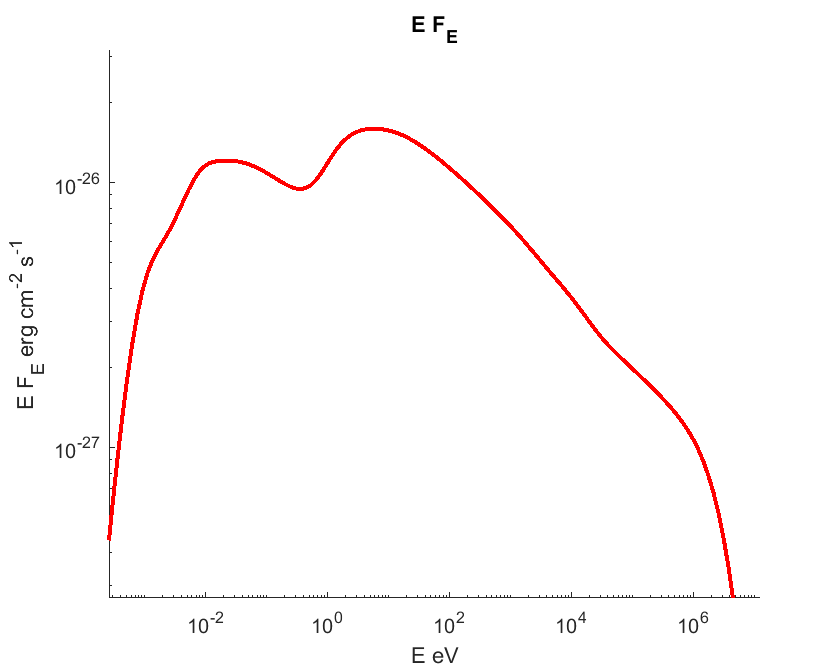
\includegraphics[width=12.5 cm]{./fig/compton.png} 
	\caption{Энергетическая плотность потока синхротронного излучения от тестового источника}
	\label{compton}
\end{figure}

\subsection{Распад пионов}

Для расчета излучения, получающегося в результате распада пионов, родившихся в результате свободно-свободного взаимодействия протонов использеутся абастрактный класс PionDecayEvaluatorBase и двае его наследника: PionDecayEvaluatorKelner, в котором сечение излучения гамма-фотона считается долей от полного сечения неупругого взаимодействия протонов, как описано в статье \cite{Kelner}, и PionDecayEvaluator, в котором используется более точное описание сечения рождения пионов на низких энергиях по методу, описанному в \cite{Kafexhiu}. В текущей версии предполагается, что характерное время потерь энергии протонов при неупругом взаимодействии намного больше времени их удержания в источнике, система является прозрачной для протонов, и каждый из них взаимодействует не более одного раза. В противном случае используемая модель излучения не применима.

При создании объекта класса PionDecayEvaluator необходимо указать рассматриваемый диапазон энергий частиц и количество точек в нем, а так же концентрацию фоновых протонов, так как предполагается рассеяние высокоэнергичных фотонов на покоящихся, а не взаимодействие высокоэнергичных между собой. Публичные методы класса PionDecayEvaluatorBase и его наследников приведены в Таблице \ref{pionDecay}

		\begin{small}
			\topcaption{Публичные методы классa PionDecayEvaluatorBase и его наследников }
			\label{pionDecay}
			\begin{xtabular}{|p{0.5\textwidth}|p{0.5\textwidth}|}  
				\hline
				\textbf{PionDecayEvaluatorBase} & абстрактный класс для вычисления гамма излучения от распада пионов\\
				\hline
				sigmaInelastic(const double\& energy) & возвращает полное сечение неупругого взаимодействия протонов в лабораторной системе, принимает кинетическую энергию движущегося протона\\
				\hline
				\textbf{PionDecayEvaluatorKelner} & класс для вычисления гамма излучения от распада пионов по методу из статьи \cite{Kelner}\\
				\hline
				PionDecayEvaluatorKelner(int Ne, double Emin, double Emax, const double\& ambientConcentration) & конструктор, создает экземпляр с заданным рассматриваемым диапазоном энергии и концентрацией фоновых протонов\\
				\hline
				\textbf{PionDecayEvaluator} & класс для вычисления гамма излучения от распада пионов по методу из статьи \cite{Kafexhiu}\\
				\hline
				PionDecayEvaluator(int Ne, double Emin, double Emax, const double\& ambientConcentration) & конструктор, создает экземпляр с заданным рассматриваемым диапазоном энергии и концентрацией фоновых протонов\\
				\hline
				sigmaGamma(const double\& photonEnergy, const double\& protonEnergy) & возвращает дифференциальное сечение рождения фотона с данной энергией при данной кинетической энергии протона, усредненное по углам\\
				\hline
			\end{xtabular}
		\end{small}

Пример вычисления излучения от гамма излучения от распада пионов показан в функции evaluatePionDecay() в файлк examples.cpp. В нем рассмотрено моделирование излучение объекта Кокон Лебедя в модели ускорения частиц на вторичных ударных волнах, следуя статье \cite{BykovKalyashova2022}. В данной работе вычислено, что спектр ускоренных протонов имеет вид степенной функции с изломом со следующими параметрами - показатели спектра 2.1 и 2.64 на низких и высоких энергиях соответственно, энергия излома - 2.2 ТэВ. Размер излучающей области брался равным размеру сверхкаверны Лебедя - 55 пк. Как и ранее, сначала определим переменные, задающие основные параметры источника - концентрацию частиц, его размер и магнитное поле, которое опять положим равным нулю. Диапазон энергий протонов рассмотрим от 0.01 ГэВ до 10 ТэВ. Так же укажем энергию излома.
\begin{lstlisting}[language=c++]
	double protonConcentration = 150;
	double rmax = 55 * parsec;
	double B = 0;
	double sinTheta = 1.0;

	double distance = 1400 * parsec;
	double Emin = massProton*speed_of_light2 + 0.01E9 * 1.6E-12;
	double Emax = 1E13 * 1.6E-12;
	double Etrans = 2.2E12 * 1.6E-12;
\end{lstlisting}
После этого создадим распределение протонов и источник излучения
\begin{lstlisting}[language=c++]
	MassiveParticleBrokenPowerLawDistribution* protons = new 
		MassiveParticleBrokenPowerLawDistribution(
		massProton, 2.1, 2.64, Emin, Etrans, protonConcentration);
	RadiationSource* source = new SimpleFlatSource(
		protons, B, sinTheta, rmax, rmax, distance);
\end{lstlisting}
Далее потребуется вычислитель излучения. В случае пионного распада необходимо указать концентрацию фоновых протонов.
\begin{lstlisting}[language=c++]
double protonAmbientConcentration = 20;
PionDecayEvaluator* pionDecayEvaluator = new PionDecayEvaluator(
	200, Emin, Emax, protonAmbientConcentration);
\end{lstlisting}
Как и в предыдущих случаях далее необходимо внутри цикла вычислить излучение в интересующем диапазоне энергий, используя функцию evaluateFluxFromSource, и вывести результат в файл в удобных единицах. Спектр излучения, полученный в результате работы данной программы и результаты наблюдений Кокона Лебедя на Fermi LAT, ARGO и HAWC \cite{Ackermann2011, Bartoli2014, Abeysekara2021} приведены на рисунке \ref{pion}
\begin{figure}
	\centering
	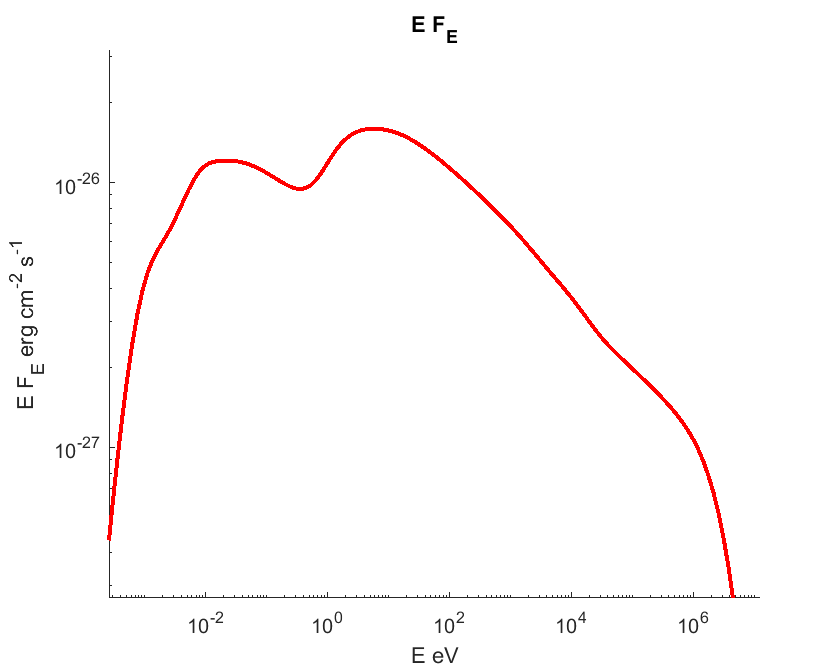
\includegraphics[width=12.5 cm]{./fig/compton.png} 
	\caption{Расчетная энергетическая плотность потока гамма излучения Кокона Лебедя и данные наблюдений}
	\label{pion}
\end{figure}
\subsection{Тормозное излучение}
В текущей версии кода реализовано вычисление тормозного излучения электронов в плазме только для случая теплового распределения. Для этого предназначен класс BremsstrahlungThermalEvaluator. В процессе расчета предполагается, что плазма электрон-протонная, с одинаковыми температурами электронов и протонов, в вычислении используются Гаунт-факторы, приведенные в \cite{Rybicki}. Пример вычисления тормохного излучения приведен в функции evaluateBremsstrahlung в файле examples.cpp.

